\documentclass[tikz,border=15pt]{standalone}
\usepackage{amsmath, amssymb}
\usetikzlibrary{positioning, arrows.meta, shapes.geometric, shapes.multipart, fit, backgrounds, decorations.pathreplacing}

% Macros from your text
\newcommand{\Z}{\mathbb{Z}}
\newcommand{\C}{\mathbb{C}}
\newcommand{\F}{\mathbb{F}}
\newcommand{\ideal}[1]{\langle #1 \rangle}
\newcommand{\Spec}{\operatorname{Spec}}
\newcommand{\im}{\operatorname{im}}
\newcommand{\Ker}{\operatorname{Ker}}
\newcommand{\ol}[1]{\overline{#1}}

\begin{document}
	
	% ==========================================
	% DIAGRAM 1: The Rosetta Stone Triad
	% ==========================================
	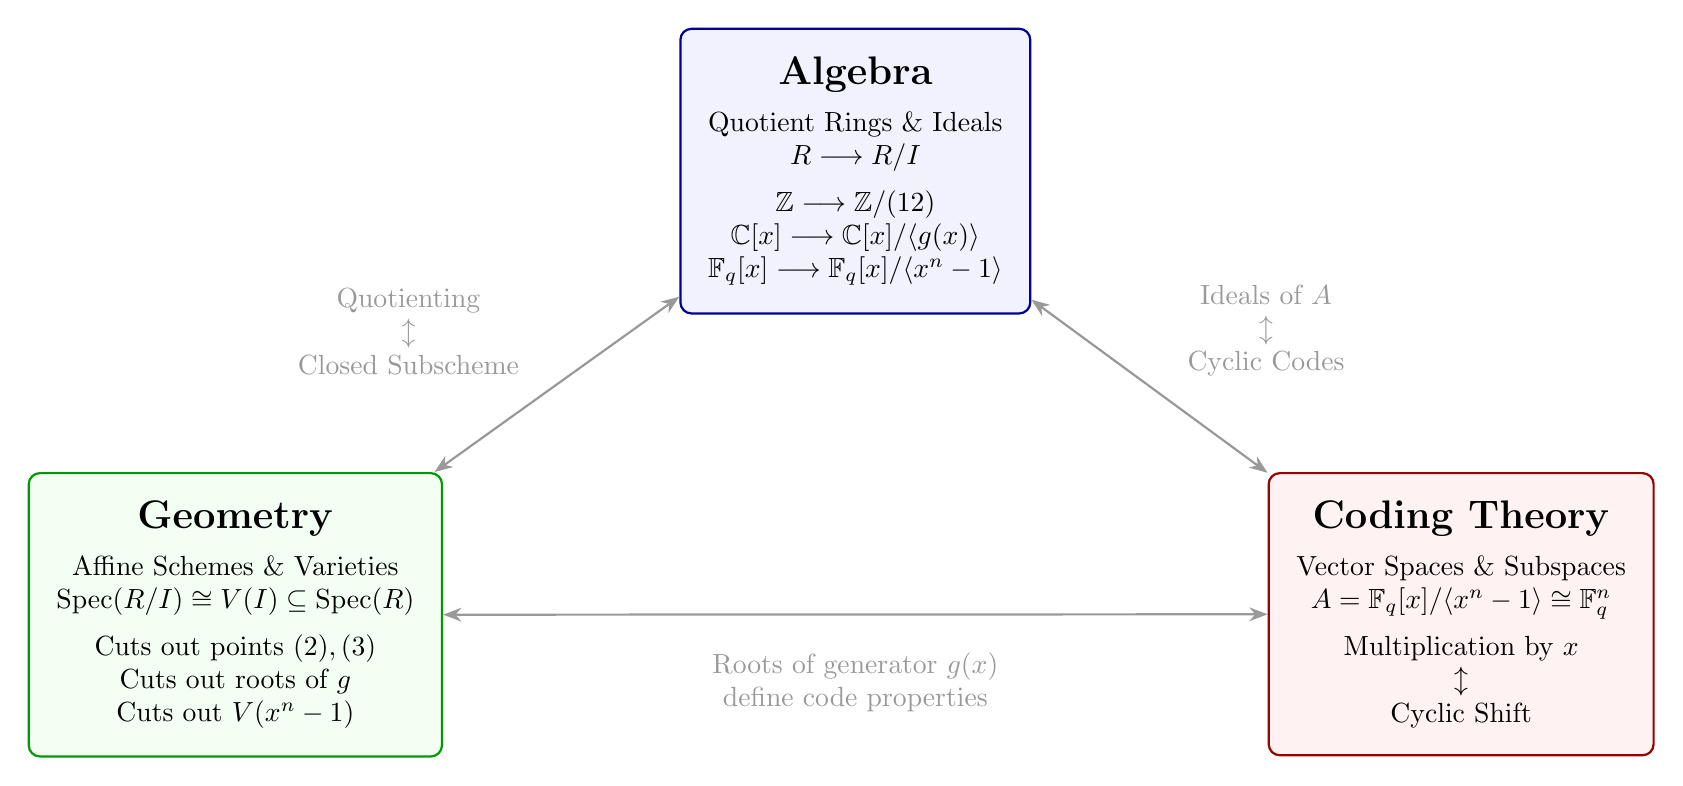
\begin{tikzpicture}[
		node distance=2cm and 3cm,
		box/.style={draw, rounded corners, align=center, thick, inner sep=10pt},
		algbox/.style={box, fill=blue!5, draw=blue!60!black},
		geobox/.style={box, fill=green!5, draw=green!60!black},
		codebox/.style={box, fill=red!5, draw=red!60!black},
		arrow/.style={-{Stealth[length=3mm]}, thick, color=gray!80},
		biarrow/.style={<->, >=Stealth, thick, color=gray!80}
		]
		
		% ALGEBRA NODE (Top)
		\node[algbox] (alg) {
			\textbf{\Large Algebra} \\[.5em]
			Quotient Rings \& Ideals \\
			$R \longrightarrow R/I$ \\[.5em]
			$\Z \longrightarrow \Z/(12)$ \\
			$\C[x] \longrightarrow \C[x]/\ideal{g(x)}$ \\
			$\F_q[x] \longrightarrow \F_q[x]/\ideal{x^n-1}$
		};
		
		% GEOMETRY NODE (Bottom Left)
		\node[geobox, below left=of alg] (geo) {
			\textbf{\Large Geometry} \\[.5em]
			Affine Schemes \& Varieties \\
			$\Spec(R/I) \cong V(I) \subseteq \Spec(R)$ \\[.5em]
			Cuts out points $(2), (3)$ \\
			Cuts out roots of $g$ \\
			Cuts out $V(x^n-1)$
		};
		
		% CODING NODE (Bottom Right)
		\node[codebox, below right=of alg] (code) {
			\textbf{\Large Coding Theory} \\[.5em]
			Vector Spaces \& Subspaces \\
			$A = \F_q[x]/\ideal{x^n-1} \cong \F_q^n$ \\[.5em]
			Multiplication by $x$ \\
			$\updownarrow$ \\
			Cyclic Shift
		};
		
		% CONNECTIONS
		\draw[biarrow] (alg) -- (geo) node[midway, above left, align=center, xshift=-10pt] {Quotienting\\$\updownarrow$\\Closed Subscheme};
		\draw[biarrow] (alg) -- (code) node[midway, above right, align=center, xshift=10pt] {Ideals of $A$\\$\updownarrow$\\Cyclic Codes};
		\draw[biarrow] (geo) -- (code) node[midway, below, align=center, yshift=-10pt] {Roots of generator $g(x)$\\define code properties};
		
	\end{tikzpicture}
	
	% ==========================================
	% DIAGRAM 2: The Cyclic Code Mechanism
	% ==========================================
	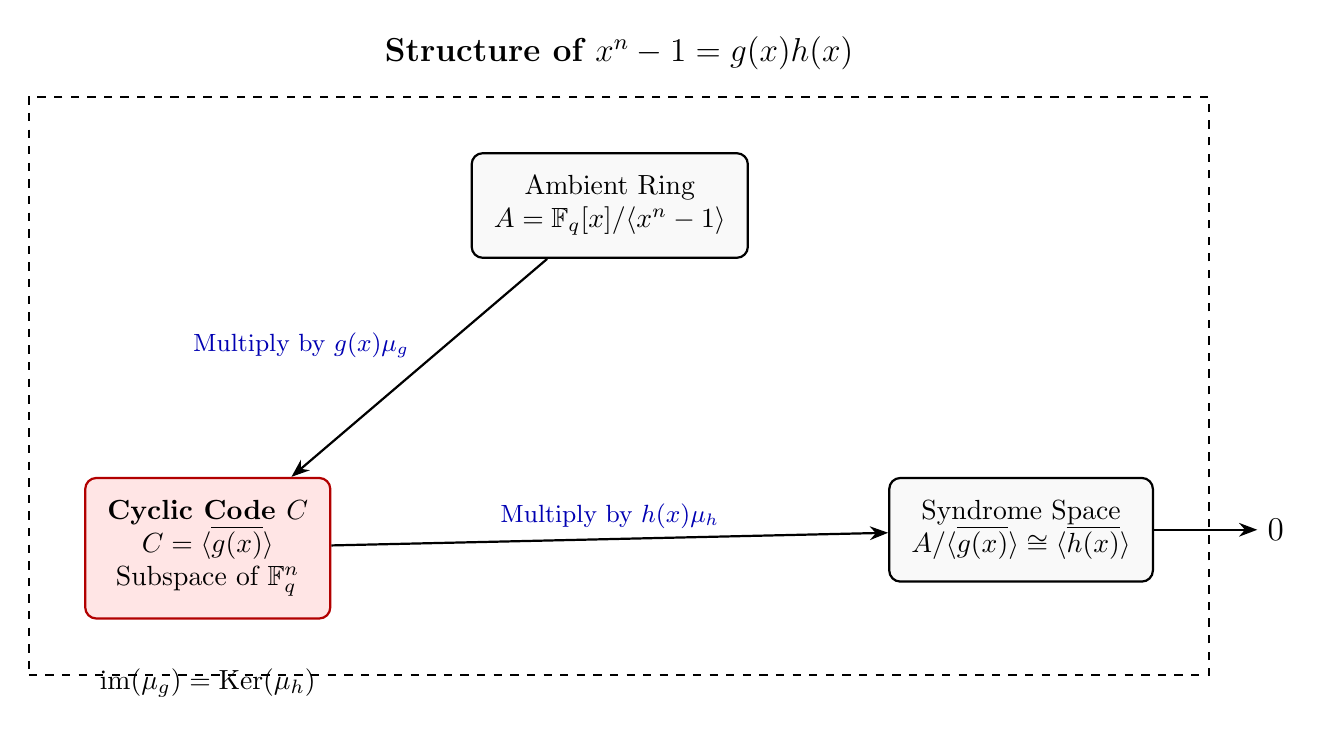
\begin{tikzpicture}[
		node distance=2.5cm,
		box/.style={draw, rectangle, rounded corners, align=center, thick, fill=gray!5, inner sep=8pt, minimum height=1cm},
		arrow/.style={->, >=Stealth, thick},
		label/.style={font=\small\color{blue!70!black}}
		]
		
		% Define Nodes
		\node[box] (A) {Ambient Ring \\ $A = \F_q[x]/\ideal{x^n-1}$};
		
		\node[box, below left=of A, yshift=-1cm, fill=red!10, draw=red!70!black] (C) {
			\textbf{Cyclic Code $C$} \\
			$C = \ideal{\ol{g(x)}}$ \\
			Subspace of $\F_q^n$
		};
		
		\node[box, below right=of A, yshift=-1cm] (Syndrome) {
			Syndrome Space \\
			$A/\ideal{\ol{g(x)}} \cong \ideal{\ol{h(x)}}$
		};
		
		% Draw exact sequence / mappings
		\draw[arrow] (A) -- (C) node[midway, above left, label] {Multiply by $g(x)$ \\ $\mu_g$};
		\draw[arrow] (C) -- (Syndrome) node[midway, above, label] {Multiply by $h(x)$ \\ $\mu_h$};
		\draw[arrow] (Syndrome) -- +(3,0) node[right, font=\large] {$0$};
		
		% Annotations
		\node[below=0.5cm of C, font=\bfseries] {$\im(\mu_g) = \Ker(\mu_h)$};
		
		% Structural Box for the final boxed equation
		\node[draw, thick, dashed, fit=(A)(C)(Syndrome), inner sep=20pt] (frame) {};
		\node[above=0.2cm of frame, font=\bfseries\large] {Structure of $x^n-1 = g(x)h(x)$};
		
	\end{tikzpicture}
	
\end{document}